\documentclass[border=0pt]{standalone} % Remove extra margins
\usepackage{tikz}
\usetikzlibrary{positioning}

\begin{document}

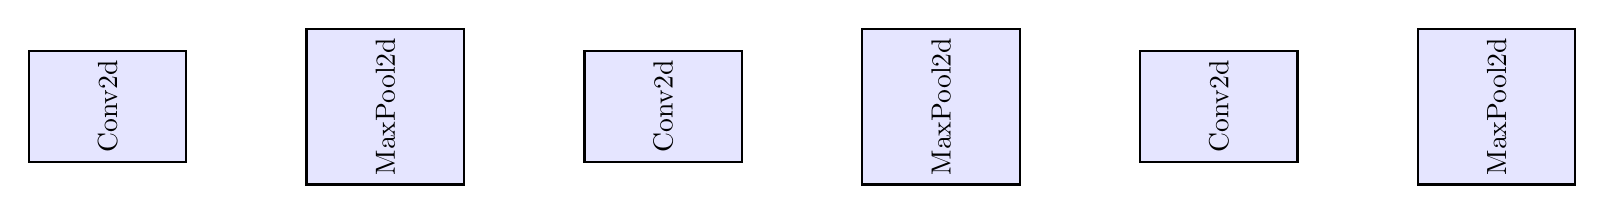
\begin{tikzpicture}[
    node distance=1.5cm, % Reduced node distance
    thick,
    layer/.style={rectangle, draw, minimum width=2cm, minimum height=1cm, fill=blue!10},
    arrow/.style={->, thick}
]

\node[layer] (conv1) {\rotatebox{90}{Conv2d}};
\node[layer, right=of conv1] (max1) {\rotatebox{90}{MaxPool2d}};

\node[layer, right=of max1] (conv2) {\rotatebox{90}{Conv2d}};
\node[layer, right=of conv2] (max2) {\rotatebox{90}{MaxPool2d}};
\node[layer, right=of max2] (conv3) {\rotatebox{90}{Conv2d}};
\node[layer, right=of conv3] (max3) {\rotatebox{90}{MaxPool2d}};

\end{tikzpicture}

\end{document}
